\documentclass{article}

\usepackage{tikz}
\usepackage[a4paper]{geometry}
\usepackage[utf8]{inputenc}
\usepackage[english]{babel}
\usepackage[noend]{algpseudocode}
\usepackage{amsthm}
\usepackage{amsmath}
\usepackage{colortbl}
\usepackage{graphicx}
\usepackage{lineno}
\usepackage[textwidth=4cm]{todonotes}
\usepackage{float}
\usepackage{amssymb}
\usepackage{subfiles}
\usepackage{xcolor}

\newcommand{\method}[1]{\textsc{#1}}

\geometry{left=3cm, right=6cm, top=3cm, bottom=3cm, marginparwidth=4cm} 

\linenumbers

\definecolor{verylightgray}{gray}{0.95}
\setuptodonotes{noline, color=green!15, size=\scriptsize}

\newtheorem*{problem}{Problem}
\newcommand{\grey}{\cellcolor{black!25}}

\title{Algorithms and Data Structures \\
  Handin 8: Reachability}

\author{
    202605673 Lukas Alstrup \\
    202605116 Thomas Seeberg Hansen \\
    202606296 Frederik Dommer Løvbjerg Plum
}

\date{23. October, 2026}  % Use \date to set a specific date

\begin{document}

\maketitle
\begin{problem}[8 Reachability]
\end{problem}

\section*{Comment}

\section*{Our solution}
Let $G=(E,V)$ be a directed graph with each vertex $v \in V$ labelled with a unique integer $L(u)$ from the set $\{1, 2, \hdots, |V| \}$. For each vertex $u \in V$ we let $R(u) = \{ v \in V : u \rightsquigarrow v\}$ be the set of verticies that are reachable from $u$. We let $min(u)$ be the vertex in $R(u)$ whose label is minimum such that: $min(u)$ is the vertex $v$ such that $L(v) = min\{L(w): w \in R(u) \}$. We wish to find an $O(V+E)$ algorithm to compute $min(u)$ for all verticies $u \in V$.




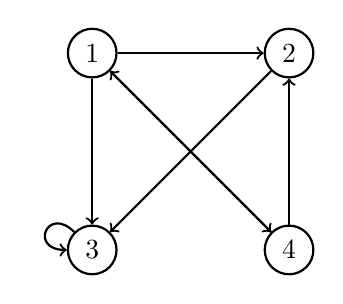
\begin{tikzpicture}[node distance={25mm}, thick, main/.style = {draw, circle}]
	\node[main] (1)  {$1$};
	\node[main] (2) [right of=1] {$2$};
	\node[main] (3) [below of=1] {$3$};
	\node[main] (4) [below of=2] {$4$};

	\draw[->] (1) -- (2);
	\draw[->] (1) -- (3);
	\draw[->] (1) -- (4);

	\draw[->] (2) -- (3);

	\draw[->]  (3) to [out=135,in=180,looseness=5] (3);

	\draw[->] (4) -- (2);
	\draw[->] (4) -- (1);

\end{tikzpicture}


\begin{center}
	\begin{minipage}{6.8cm}
		\begin{algorithmic}
			\Procedure{dfs}{G}
			\State byLabel = new Node[G.length]
			\For{u \textbf{in} G}
			\State byLabel[u.uniqueInteger - 1] = u
			\EndFor

			\For{u \textbf{in} byLabel}
			\If{u.color == "white"}
			\State{dfs-visit(u, u.uniqueInteger)}
			\EndIf
			\EndFor
			\EndProcedure
		\end{algorithmic}
	\end{minipage}
\end{center}


\begin{center}
	\begin{minipage}{6.8cm}
		\begin{algorithmic}
			\Procedure{dfs-visit}{G}
			\State{u.color = "black"}
			\State{u.minValue = label}

			\For{v \textbf{in} u.parents}
			\If{v.color == "white" }
			\State{dfs-visit(v, label)}
			\EndIf
			\EndFor{}
			\EndProcedure
		\end{algorithmic}
	\end{minipage}
\end{center}


\end{document}
